% Metódy inžinierskej práce

\documentclass[10pt,twoside,slovak,a4paper]{article}

\usepackage[slovak]{babel}
%\usepackage[T1]{fontenc}
\usepackage[IL2]{fontenc} % lepšia sadzba písmena Ľ než v T1
\usepackage[utf8]{inputenc}
\usepackage{graphicx}
\usepackage{url} % príkaz \url na formátovanie URL
\usepackage{hyperref} % odkazy v texte budú aktívne (pri niektorých triedach dokumentov spôsobuje posun textu)

\usepackage{cite}
%\usepackage{times}

\pagestyle{headings}

\title{Adaptívna personalizovaná gamifikácia vo vzdelávacích prostrediach\thanks{Semestrálny projekt v predmete Metódy inžinierskej práce, ak. rok 2022/23, vedenie: Ing. Fedor Lehocki, PhD}} % meno a priezvisko vyučujúceho na cvičeniach

\author{Daniel Štilec\\[2pt]
	{\small Slovenská technická univerzita v Bratislave}\\
	{\small Fakulta informatiky a informačných technológií}\\
	{\small \texttt{xstilec@stuba.sk}}
	}

\date{\small 30. september 2022} % upravte



\begin{document}

\maketitle

\begin{abstract}
Gamifikácia je trend, ktorý sa zaoberá aplikáciou herných prvkov napríklad do vzdelávacích prostredí so záujmom zvýšenia produktivity používateľa. Cieľom gamifikácie je zabaviť, motivovať, ale hlavne naučiť. Avšak je vždy gamifikácia účinná? Nie každý herný prvok môže byť vhodný pre daného používateľa a to môže viesť k strate motivácie do vzdelávania. Nasledujúci článok sa bude zaoberať pojmom personalizovaná gamifikácia a ako ju implementovať do vzdelávacích aplikácií s cieľom zvýšenia motivácie a produktivity používateľov.
\end{abstract}


\section{Personalizácia} \label{personalizacia}

%\centering
%\includegraphics[scale=1.0]{diagram.pdf}
	Personalizácia je pojem, ktorý v modernom svete stále nie je tak populárny ako by mal byť. Slovenské školy, či už je to základná, stredná alebo vysoká škola, uprednostňujú rovnaký spôsob vzdelávania. Stanovené učebné plány a rozvrhy nemusia sedieť každému. Samozrejme, existujú úľavy pre študentov a žiakov s rôznymi disfunkciami, ale to neznamená, že škola je personalizovaná a adaptuje sa študentom. Hlavným znakom personalizovaného vzdelávania je postavenie sa ku každému osobitne.

\subsection{Personalizovaná gamifikácia} \label{personalizacia:gamifikacia}

	Existuje spôsob ako by sa študenti mohli zlepšovať vo svojich záujmoch, ako by mohli zostať stále motivovaní, pretože to patrí medzi najdôležitejšie atribúty vzdelávania. Personalizovaná gamifikácia skúma potreby a chovanie sa používateľa s výsledkom prispôsobenia herných prvkov jednotlivcom \cite{personalizovana} .Napríklad niektoré vzdelávacie aplikácie by mohli zmeniť sadu herných prvkov A na sadu prvkov B ak sú používatelia ženy, pretože ženám nemusí vždy vyhovovať to, čo mužom. V skratke, ľudia z rôznych štátov, etnických skupín, spoločností, ktorí majú rozličné charakteristiky sú motivovaní odlišne a preto by gamifikované systémy mali byť špecificky prispôsobené rôznym používateľom aby gamifikácia naplno využila svoj potenciál. 


\section{Aplikácie s využitím personalizovanej gamifikácie} \label{aplikacie}

\subsection{Duolingo} \label{aplikacie:duolingo}

Duolingo je bezplatná aplikácia, ktorá pomáha naučiť sa cudzí jazyk alebo sa v ňom zdokonaliť. Používa jedinečný adaptívny systém, ktorý sleduje úroveň znalostí každého jednotlivca. Taktiež zbiera informácie o slovách ktoré môžu byť ťažšie zapamätateľné a tieto informácie posúva ďalším používateľom. Duolingo myslí aj na možnosť, keď používateľ môže po čase niečo zabudnúť a tak mu danú časť výučby môže zopakovať. \cite{duolingo}

\subsection{Knewton} \label{aplikacie:knewton}

Knewton je vzdelávací systém zameraný na poskytovanie individualizovaného a neustále sa prispôsobujúceho prostredia a zároveň poskytuje okamžitú spätnú väzbu, gamifikačné komponenty a sociálnu zložku, kde môžu študenti spolupracovať. \cite{knewton} Systém je vytvorený implementáciou niekoľkých výkonných matematických modelov, ako je teória odozvy na položky, Bayesovské siete, Markovove modely a klastrovacie algoritmy. Všetky tieto metódy sa používajú na hodnotenie vedomostí študentov, vytváranie personalizovaných ciest a hľadanie vzorov v skupinách študentov.

\section{Prieskum} \label{prieskum}

Tento článok vychádza z prieskumu\cite{adaptiveGamification}, ktorý bol smerovaný na skupinu vysokoškolákov, ktorý navštevujú kurzy vývoja internetových stránok. Účastníci prieskumu museli vyjadriť svoj postoj k trom základným otázkam (viď Obr. 1 \ref{fig: tabulka} ), a to:
\begin{enumerate}
\item Je personalizovaný prístup efektívnejší ako prístup, ktorý je rovnaký pre všetkých študentov ?
\item Pomôže adaptívne testovanie posilniť vedomosti ? 
\item Posilnia prvky gamifikácie motiváciu a zábavu študentov pri učení ? 
\end{enumerate}

\begin{figure}[h]
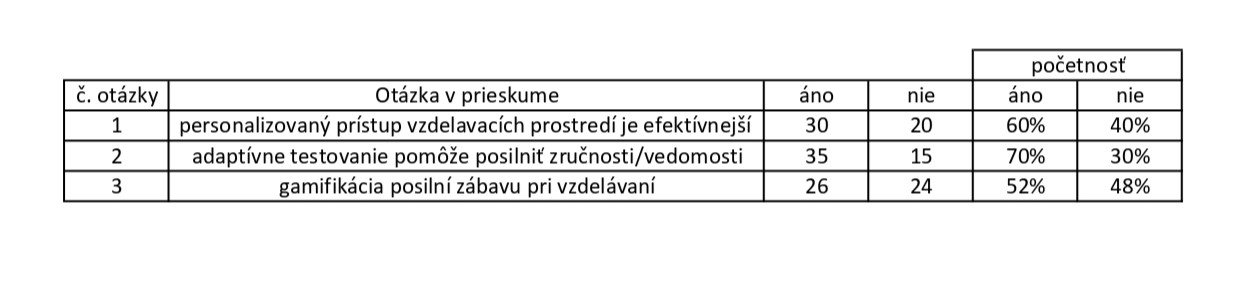
\includegraphics[scale=.75]{tabulka.jpg}
\label{fig: tabulka}
\caption{Tabuľka popisuje odpovede na otázky v prieskume. Na prieskume sa celkovo zúčastnilo 50 študentov vysokej školy.}
\end{figure}

Na základe toho prieskumu sa zistilo, že je potrebné vytvoriť vzdelávacie prostredie, ktoré je jednoduché na používanie, kde používatelia majú voľnosť a priestor na chyby počas vzdelávania. Taktiež bolo pre túto skupinu ľudí dôležité aby systém obsahoval bodovanie výkonu používateľa.

Na základe výsledkov prieskumu je nutné aby systém obsahoval nasledovné: 
\begin{itemize} \label{prvky}
\item jednoduché a pochopiteľné rozhranie
\item jasne definovaný obsah vzdelávania
\item výber náročnosti
\item opätovné použitie otázok na zistenie vedomostí
\item herné prvky \cite{duolingo} - úrovne, počítadlo bodov
\item kompatibilita s mobilným zariadením
\end{itemize}

Hlavnou vlastnosťou, čo systém potrebuje obsahovať je adaptivita. Implementáciou opätovného použitia testovacích otázok sa docieli zber informácií o aktuálnom leveli vedomostí, ktoré budú neskôr použité na výber testovacích otázok. Opätovné použitie otázky je spôsob, akým systém reaguje na používateľa po nesprávnej alebo správnej odpovedi, pričom je prezentovaná rovnaká otázka s rôznym výberom odpovedí.

\section{Základná kostra programu} \label{program}

V nasledujúcej sekcii článok opíše základnú kostru (viď obr.2 \ref{fig: diagram} ) a správanie programu na vzdelávanie, ktorý obsahuje personalizovanú gamifikáciu.

\begin{figure}[h]
\includegraphics[scale=.55]{diagram_prezentácia.pdf}
\label{fig: diagram}
\caption{Diagram opisuje správanie programu}
\end{figure}

Po spustení programu má používateľ na výber z ponúkaných vzdelávacích tém spolu s voľbou náročnosti. Zvolením témy sa používateľovi zobrazí prvá testovacia otázka. Ako ďalší krok program vyhodnocuje odpoveď na danú otázku. Ak používateľ odpovedal správne pripíšu sa body za správnu odpoveď a program pokračuje na ďalšiu otázku. Na druhú stranu ak používateľ odpovedal nesprávne, program si túto testovaciu otázku zapamätá a v ďalšom teste s rovnakou témou sa použije znova, ale so zmenenou náročnosťou. To znamená, ak mal používateľ v teste zapísať správne odpoveď a nezvládol to, v nasledujúcom teste bude mať na výber z možností odpovedi a podobne.

\section{Prvotný model programu} \label{prototyp} 

Prvotný model programu bol predložený osemnástim študentom na testovanie. Je dôležité si uvedomiť, že ide o prvotný model a tým pádom bola v programe na výber len jedna vzdelávacia téma. Z toho vyplýva, že všetci študenti boli testovaní práve na jednej vzdelávacej téme. Testovanie programu sa dá rozdeliť na dve fázy: 

\begin{enumerate}
\item Prvé použitie programu, kde zúčastnení nemali predtým s programom žiadny styk.
\item Opätovné použitie s odstupom času.
\end{enumerate}
\subsection{Prvé použitie programu} \label{prvePouzitie}
Pri úplne prvom styku s programom bola viac ako polovica študentov schopná získať viac ako 50 skúsenostných bodov a niektorý dokonca prešli na úroveň 2, čiže získali 100 skúsenostných bodov. Keďže každá správna odpoveď je ohodnotená 10 bodmi študenti v priemere odpovedali správne na 5 až 10 otázok.

\subsection{Opätovné použitie programu} \label{dalsiePouzitie}
Nasleduje fáza opätovného použitia programu. Niektorým z predošlých študentov bola predložená rovnaká vzdelávacia téma ako v prvej fáze. 
Týmto študentom sa podarilo získať 350 skúsenostných bodov, čo je najvyššie možné ohodnotenie ktoré mohli v prvotnej verzii získať.

\subsection{Poznatky}
Zo zaznamenaných výsledkov z opätovného použitia môžeme predpokladať, že personalizovaná gamifikácia splnila svoj účel. Spomínané prvky gamifikácie \ref{prieskum} mali za následok zvýšenie motivácie používateľov a taktiež vytvorili príjemné vzdelávacie prostredie kam sa študenti chceli opäť vrátiť a naučiť sa niečo nové.

\section{Záver}

Personalizovaná gamifikácia je pojem, ktorý by mal zaujímať každú firmu alebo jednotlivca, ktorý vytvára určitú službu pre ľudí v digitálnom svete. Jej vlastnosti jednoznačne vytvoria príjemné prostredie pre jednotlivcov, ktoré je do určitej miery "ušitý na mieru" svojmu používateľovi. Personalizovaná gamifikácia sa dá využiť v mnoho smeroch a tento článok sa zaoberal tým, ako zaviesť personalizovanú gamifikáciu do vzdelávacieho prostredia. Článok neposkytuje podrobný návod ako naprogramovať systém, ktorý obsahuje personalizovanú gamifikáciu, ale len stručné vyjadrenie základných vlastností a princípov gamifikovaného systému spolu s personalizáciou.

\section{Reakcia na témy z prednášok}

\subsection{Udržateľnosť a etika}

Na prednáške s názvom Udržateľnosť a etika sme sa zaoberali pojmom udržateľnosť ako zotrvačnosť ktorá nie je dôležitá len pri osobnom raste ľudí, ale je dôležitá aj keď hovoríme o prednáškach. Prednášajúci profesor viedol diskusiu o tom ako docieliť udržateľnosť na prednáškach. Podľa mňa udržateľnosť na prednáškach ovplyvňuje množstvo faktorov. Napríklad dĺžka prednášky, prístup prednášajúceho, práca s hlasom a taktiež obsah prednášok. Najdôležitejšie je, aby prednášajúci vytvoril prednášku ktorá sa drží stanovených študijných osnov, ale aj aby priniesol študentom kvalitné, zaujímavé a zábavné spracovanie témy.

\subsection{Grafické vyjdrenie informácií v informatike}

Na štvrtej prednáške sme sa venovali téme prečo je vizualizácia v informatike dôležitá. Oboznámili sme sa s výrokom \textit{"Počujem a zabudnem. Vidím a pamätám. Robím a rozumiem."} od čínskeho filozofa Konfucia. S výrokom plne súhlasím, podľa mňa je správne grafické spracovanie veľmi dôležité. Pre mňa ako človeka, ktorý sa v budúcnosti chce zaoberať programovaním webových stránok a aplikácií a taktiež ich dizajnom, je dôležité aby som apeloval na správne grafické spracovanie. Budem si dávať pozor na použitie správnych farieb, to aby som poskytol len tie najdôležitejšie informácie a ďalšie aspekty.

\subsection{Prezentácia: slajdy a prednes}

Na tejto prednáške sme sa venovali ako správne prezentovať prezentáciu, čomu sa vyhnúť, a čo na druhú stranu je dôležité robiť pri prezentáciách. Sám na sebe vidím, že občas robím chyby pri prezentácii a najmä to, že nedodržiavam očný kontakt, čo plynie hlavne z trémy pred ľuďmi. Napriek mojim chybám sa mi páči, že dokážem publiku podať informácie jednoducho, aby to bolo ľahké na zapamätanie a aby som nepôsobil nudne.

% týmto sa generuje zoznam literatúry z obsahu súboru literatura.bib podľa toho, na čo sa v článku odkazujete
\bibliography{lit}
\bibliographystyle{plain} % prípadne alpha, abbrv alebo hociktorý iný
\end{document}
